
\chapter{Algorithm}

To write pseudocode algorithms, you should use several packages:
\lstset{language=TeX}
\begin{lstlisting}
  \usepackage[ruled,vlined]{algorithm2e}
\end{lstlisting}


\section{Example}

\begin{lstlisting}

  \begin{algorithm}[H]
    \SetAlgoLined
    \KwData{this text}
    \KwResult{how to write algorithm with \LaTeX2e }
    initialization\;
    \While{not at end of this document}{
      read current\;
      \eIf{understand}{
        go to next section\;
        current section becomes this one\;
      }{
        go back to the beginning of current section\;
      }
    }
    \caption{How to write algorithms}
  \end{algorithm}

\end{lstlisting}


The result is shown in Figure \ref{fig:algorithm2e-example}
\begin{figure}[H]
  \centering
  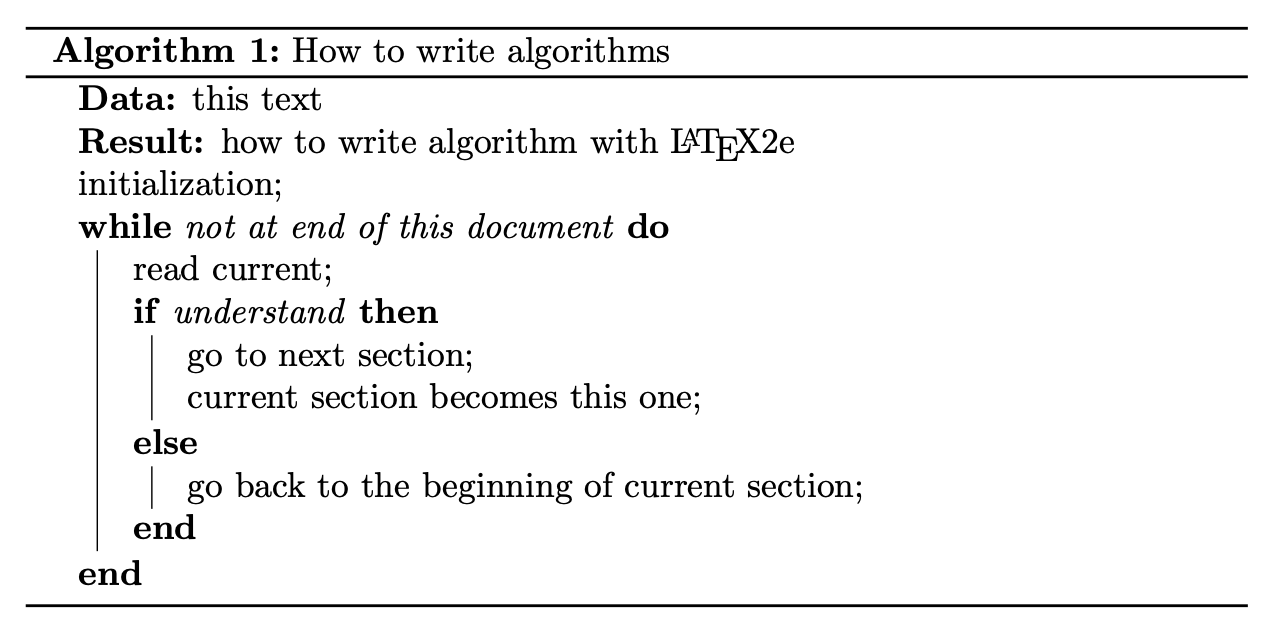
\includegraphics[width=\textwidth]{algorithm2e-example}
  \caption{Algorithm2e example}
  \label{fig:algorithm2e-example}
\end{figure}